\chapter{Koncepcja rozwiązania}

W niniejszym rozdziale skupiam się na opisie koncepcji rozwiązania wykorzystania
analizy sentymentu, sieci społecznych i geolokacji w analizie zachowań
użytkowników serwisów społecznościowych. W kolejnych podrozdziałach opisuję
sposoby w jaki dane zagadnienia zostały zaaplikowane w moich badaniach.
Na początku przedstawiam gruboziarnisty model systemu (\ref{section:modelsystemu}),
który prezentuje jego najważniejsze moduły. Następnie opisuję tematykę
i sposób gromadzenia danych (\ref{section:gromadzeniedanych}) potrzebnych do 
przeprowadzenia analizy internautów. Później omawiam metodę jaką zastosowałem 
podczas analizy sentymentu (\ref{section:analizasentymentu}) wpisów użytkowników.
W dalszej kolejności skupiam się nad zastosowanymi
sposobami analizy sieci społecznych (\ref{section:siecispoleczne})
i całość kończę omówieniem wykorzystania geolokacji w moich badaniach 
(\ref{section:wykorzystaniegeolokacji}).








%%%%%%%%%%%%%%%%%%%%%%%%%%%%%%%%%%%%%%%%%%%%%%%%%%%%%%%%%%%%%%%% MODEL SYSTEMU
\section{Model systemu}
\label{section:modelsystemu}
Stworzony przeze mnie system składa się z kilku modułów. Trzy najważniejsze
z nich to:
\begin{itemize}
  \item gromadzenie danych,
  \item przetwarzanie danych,
  \item analiza zebranych danych.
\end{itemize}
Wszystkie dane gromadzone są w jednej bazie danych.
Gruboziarnisty model systemu przedstawiony został na rysunku 
\ref{image:gruboziarnisty-model-systemu}.
\clearpage

\begin{figure}[ht!]
\centering
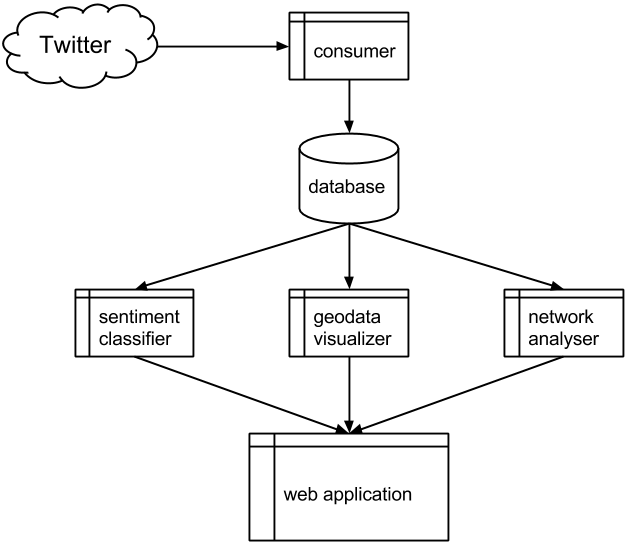
\includegraphics[width=160mm]{img/budowa-systemu.png}
\caption{Gruboziarnisty model systemu}
\label{image:gruboziarnisty-model-systemu}
\end{figure}

%%%%%%%%%%%%%%%%%%%%%%%%%%%%%%%%%%%%%%%%%%%%%%%%%%%%%%%%%%%% GROMADZENIE DANYCH
\section{Gromadzenie danych}
\label{section:gromadzeniedanych}
\subsection{Tematyka danych}
% piłka nożna, kibice
\subsection{Sposób zbierania danych}
% słowa kluczowe, API, nasłuchiwanie
\subsection{Podstawowe statystyki danych}


\clearpage
%%%%%%%%%%%%%%%%%%%%%%%%%%%%%%%%%%%%%%%%%%%%%%%%%%%%%%%%%%%% ANALIZA SENTYMENTU
\section{Analiza sentymentu}
\label{section:analizasentymentu}

\subsection{Normalizacja tekstu}
% pozbycie się słów kluczowych, zaprzeczenia, retweety
\subsection{Algorytm i jego modyfikacja}
% + dobór parametrów
\subsection{Aplikacja analizy sentymentu}
% przykładowe zdania i ich sentyment



%%%%%%%%%%%%%%%%%%%%%%%%%%%%%%%%%%%%%%%%%%%%%%%%%%%%% ANALIZA SIECI SPOŁECZNYCH
\section{Analiza sieci społecznych}
\label{section:siecispoleczne}
\subsection{Model grafowy}
% wykorzystanie reply, retweet
\subsection{Wykrywanie grup}
% gephi, modularity
\subsection{Badanie podobieństwa}
% algorytm podobieństwa grafów, podobieństwa krawędzi




%%%%%%%%%%%%%%%%%%%%%%%%%%%%%%%%%%%%%%%%%%%%%%%%%%%%%% WYKORZYSTANIE GEOLOKACJI
\section{Wykorzystanie geolokacji}
\label{section:wykorzystaniegeolokacji}
% tweety z geolokacją
% wyciąganie informacji o miejscu - Open Street Map
% zastosowanie: odl. między użytkownikiami, od stadionu, dzielnice